% !TEX TS-program = xelatex
% !TEX encoding = UTF-8 Unicode
\documentclass[letterpaper,6pt]{article}
\usepackage{amssymb} % needed for math
\usepackage{amsmath} % needed for math
\usepackage[margin=1.5cm]{geometry} %layout
\usepackage{listings} % needed for the inclusion of source code



\usepackage{float}
\usepackage{tabularx,boxedminipage}
\usepackage[cm-default]{fontspec}
\usepackage{xunicode}
\usepackage{xltxtra}
\usepackage{amssymb}
\usepackage{amsmath}
\usepackage[table,xcdraw]{xcolor}
\usepackage{algorithm}
\usepackage{algpseudocode}
\usepackage{fullpage}
%\renewcommand{\baselinestretch}{2}
\usepackage{enumerate}
\usepackage{wrapfig}
%\usepackage{xgreek}
\setmainfont{CMU Serif}
\setsansfont{CMU Sans Serif}
\newfontfamily{\greekfont}{CMU Serif}
\newfontfamily{\greekfontsf}{CMU Sans Serif}
\usepackage{graphicx}
\usepackage{polyglossia}
\setmainlanguage{greek}
\usepackage{microtype}
\usepackage{typearea}
\usepackage{booktabs}
\usepackage[makeroom]{cancel}
\usepackage{mathtools}
\usepackage{listings}
% the following is needed for syntax highlighting
\usepackage{color}

\definecolor{dkgreen}{rgb}{0,0.6,0}
\definecolor{gray}{rgb}{0.5,0.5,0.5}
\definecolor{mauve}{rgb}{0.58,0,0.82}
\DeclarePairedDelimiter\ceil{\lceil}{\rceil}
\DeclarePairedDelimiter\floor{\lfloor}{\rfloor}
% this is needed for forms and links within the text
\usepackage[hidelinks=true]{hyperref}
\newenvironment{definition}[1][Συνθήκη]{\begin{trivlist}
\item[\hskip \labelsep {\bfseries #1}]}{\end{trivlist}}
\newenvironment{lemma}[1][Λήμμα]{\begin{trivlist}
\item[\hskip \labelsep {\bfseries #1}]}{\end{trivlist}}
\newenvironment{proof}[1][Απόδειξη]{\begin{trivlist}
\item[\hskip \labelsep {\bfseries #1}]}{\end{trivlist}}
%%%%%%%%%%%%%%%%%%%%%%%%%%%%%%%%%%%%%%%%%%%%%%%%%%%%%%%%%%%%%%%%%%%%%%
% PDF Meta information                                               %
%%%%%%%%%%%%%%%%%%%%%%%%%%%%%%%%%%%%%%%%%%%%%%%%%%%%%%%%%%%%%%%%%%%%%%
\hypersetup{
  pdfauthor   = {},
  pdftitle    = {Έγγραφο ανάλυσης απαιτήσεων}
} 

\hypersetup{
    colorlinks=false,
    pdfborder={0 0 0},
}

\usepackage{tkz-graph}
\thispagestyle{empty}
%%%%%%%%%%%%%%%%%%%%%%%%%%%%%%%%%%%%%%%%%%%%%%%%%%%%%%%%%%%%%%%%%%%%%%
% THE DOCUMENT BEGINS                                                %
%%%%%%%%%%%%%%%%%%%%%%%%%%%%%%%%%%%%%%%%%%%%%%%%%%%%%%%%%%%%%%%%%%%%%%
\begin{document}
\title{Έγγραφο ανάλυσης απαιτήσεων - Τεχνολογία Λογισμικού}
\author{
  Γιώργος Δημητρακόπουλος (03113211), Χρήστος Αναγνώστου (03113166) \\
  Γιώργος Στάθης (03113008), Μάνος Πιτσιδιανάκης (03113635) \\ Ξενοφών Τσέκας (03113120), Ηλέκτρα Σκεπετάρη (03113074) \\
Κατερίνα Κουτσούρη (03113107)
}
\maketitle
\tableofcontents{}
\section{Σκοπός του συστήματος}

\subsection{Διατύπωση Προβλήματος}

Την παρούσα χρονική στιγμή, οι υπηρεσίες που προσφέρουν δραστηριότητες σε παιδιά, συντηρούνται αποσπασματικά και δεν προσφέρουν τη δυνατότητα κράτησης ή αγοράς εισιτηρίων. Με τον τρόπο αυτό δεν είναι εφικτή η άντληση, παρακολούθηση και επικαιροποίηση του συνόλου των προσφερόμενων υπηρεσιών. Οποιαδήποτε ιστοσελίδα σχετικά με παιδικές δραστηριότητες, είναι άναρχα φτιαγμένη και σπανίως συντηρείται. Ειδικότερα στην ευρύτερη περιοχή της Αθήνας, δεν υπάρχει αντίστοιχη υπηρεσία.

\subsection{Το σύστημα}

Στόχος του παρόντος συστήματος είναι η συλλογή παιδικών δραστηριοτήτων σε μια ολοκληρωμένη διαδικτυακή πλατφόρμα με σκοπό τη γεφύρωση του ψηφιακού χάσματος μεταξύ γονέων και παρόχων. Το σύστημα δίνει στους γονείς τόσο τη δυνατότητα επιλογής δραστηριοτήτων για τα παιδιά τους όσο και την κράτηση αυτών, ενώ παρέχονται διαφορετικές επιλογές ανάλογα με την ηλικία του παιδιού ή το είδος δραστηριότητας.

Οι πάροχοι δραστηριοτήτων θα ενημερώνουν την κεντρική βάση δεδομένων μέσω κατάλληλων διεπαφών που θα υλοποιηθούν στο πλαίσιο του έργου. Οι χρήστες-πάροχοι της πλατφόρμας μπορούν να διαφημίσουν την υπηρεσία τους, ενώ οι ενδιαφερόμενοι γονείς μπορούν να αναζητούν και να επιλέγουν την υπηρεσία που επιθυμούν.

Το σύστημα θα πρέπει να είναι απλό, εύχρηστο (user friendly), ώστε ο χρήστης να μπορεί να το χρησιμοποιήσει χωρίς να έχει τεχνικές γνώσεις.


\subsection{Βιωσιμότητα και αναμενόμενα οφέλη}

\subsubsection{Γονείς}

%- Coin miner js αντι διαφημίσεις

Όλες οι συναλλαγές στην ιστοσελίδα θα πραγματοποιούνται μέσω του συστήματος πόντων Coins. Οι πόντοι θα αγοράζονται από τον χρήστη μετατρέποντας με 1:150 αναλογία με το Ευρώ (€) και θα αποθηκεύονται στο ηλεκτρονικό πορτοφόλι του κάθε Γονέα-χρήστη. Δεν θα επιτρέπεται μετατροπή από Coin σε ευρώ. Οι αγόρες Coin θα γίνονται με το ακόλουθο σχήμα τιμών:

\begin{enumerate}
  \item 5€ $\to{}$ 750 coins
  \item 10€ $\to{}$ 1500 coins
  \item 20€ $\to{}$ 3000 + 75 coins
  \item 50€ $\to{}$ 7500 + 150 coins
\end{enumerate}

Παράλληλα με το σύστημα πόντων θα υπάρχει πρόγραμμα επιβράβευσης συναλλαγών με πόντους. Με αγορές αξίας 7500 πόντων ο κάθε χρήστης θα λαμβάνει 200 coins.

%~~Loot crates~~

\subsubsection{Πάροχοι}

Σε κάθε συναλλαγή θα υπάρχει προμήθεια 5\% %ή 7\% εφόσον ο πάροχος επιλέξει να προωθήσει τη συγκεκριμένη δραστηριότητα)
για τα έξοδα λειτουργίας του συστήματος καθώς και το κέρδος της επιχείρησης.

Τα αναμενόμενα οφέλη από την υλοποίηση του έργου είναι
\begin{itemize}
  \item Δημιουργία και λειτουργία ενιαίας πλατφόρμας υπηρεσιών παιδικών δραστηριοτήτων της χώρας
   \item Βελτίωση της ποιότητας και επικαιροποίηση της πληρότητας της πληροφορίας που είναι διαθέσιμη στους πολίτες, ανά γεωγραφική περιοχή της χώρας
   \item Παροχή ενός απλούστερου περιβάλλοντος δραστηριοποίησης στις επιχειρήσεις εκείνες που επιθυμούν να ενταχθούν  στο σύστημα
   \item Βελτίωση της ποιότητας των προσφερόμενων υπηρεσιών προς τους πολίτες εξυπηρετώντας βασικές ανάγκες τους και επιφέροντας σημαντικά οφέλη στον κλάδο όπως: \begin{itemize}
  \item Αναζήτηση και διαχείριση πληροφορίας με ολοένα αυξανόμενο όγκο
    \item Διατήρηση χρήσιμης πληροφορίας στο χρόνο
    \item Ηλεκτρονική διάθεση πληροφοριών και υπηρεσιών στον πολίτη
    \item Εκσυγχρονισμός του τομέα
\end{itemize}
\end{itemize}

\section{Κατηγορίες χρηστών (Users \& Stakeholders)}

    \subsection{Ανώνυμοι χρήστες}
Οι ανώνυμοι χρήστες δεν έχουν δικαίωμα αγοράς εισιτηρίων, μπορούν όμως να πλοηγούνται στις εκδηλώσεις, και να εγγραφούν στις κατηγορίες 'Γονέας' ή 'Πάροχος'. Το ρόλο του ανώνυμου χρήστη λαμβάνει όποιος εισέρχεται στην ιστοσελίδα για πρώτη φορά, ή δεν έχει ταυτοποιηθεί στο σύστημα. 

\subsection{Οι εγγεγραμμένοι χρήστες}
\subsubsection{Γονείς}
Ένας χρήστης για να εγγραφεί στο σύστημα ως 'Γονέας' θα πρέπει να καταχωρήσει τα ακόλουθα στοιχεία σε μια ειδική φόρμα εγγραφής για 'Γονείς':
\begin{itemize}
  \item Ονοματεπώνυμο
  \item Τηλέφωνο
  \item e-mail
  \item Διεύθυνση
  \item Κωδικός Ταυτοποίησης
\end{itemize}
Μετά της εγγραφή του ο γονέας μπορεί στο συνδεθεί στο σύστημα με το email και τον κωδικό ταυτοποίησης που έδωσε κατά την εγγραφή του. Ο γονέας μπορεί να αναζητήσει την υπηρεσία που τον ενδιαφέρει ανά γεωγραφική περιοχή καθώς και τους παρόχους που τις προσφέρουν. Επιπλέον, ο γονέας μπορεί να επιλέξει να προχωρήσει στην αγορά coins τα οποία στη συνέχεια μπορεί να τα εξαργυρώσει για την αγορά κάποιας υπηρεσίας. Ακόμη, στον λογαριασμό του γονέα φαίνεται το ιστορικό των αγορών του. 
\subsubsection{Πάροχοι}
Ένας χρήστης για να εγγραφεί στο σύστημα ως 'Πάροχος' θα πρέπει να καταχωρήσει τα ακόλουθα στοιχεία σε μια ειδική φόρμα εγγραφής για 'Πάροχοι':
\begin{itemize}
  \item Ονοματεπώνυμο
  \item Τηλέφωνο
  \item e-mail
  \item Διεύθυνση
  \item Κωδικός Ταυτοποίησης
  \item ΑΦΜ
  \item ΔΟΥ
  \item Νόμιμος Εκπρόσωπος
  \item Στοιχεία ταυτότητας νομίμου εκπροσώπου
  \item Ιστοσελίδα (προαιρετικά)
\end{itemize}
%Μετά την συμπλήρωση της φόρμας, αποστέλλεται στο νομικό τμήμα της εταιρείας το αίτημα ένταξης στο σύστημα ως πάροχος υπηρεσιών και ο χρήστης αποκτά έναν ανενεργό λογαριασμό. Εν συνεχεία, του αποστέλλεται ένα έγγραφο με τα στοιχεία τα οποία κατέθεσε και το συμβόλαιο συνεργασίας το οποίο καλείται να επιστρέψει υπογεγραμμένο μαζί με αντίγραφο της ταυτότητας του νομίμου εκπροσώπου της επιχείρησης ώστε να γίνει επιβεβαίωση των στοιχείων και να ενταχθεί στη λίστα παρόχων της υπηρεσίας.

Μετά την εγγραφή του, ο λογαριασμός του παρόχου ενεργοποιείται και μπορεί στο συνδεθεί στο σύστημα με το email και τον κωδικό ταυτοποίησης που έδωσε κατά την εγγραφή του.

Κατά τη σύνδεση στο λογαριασμό του, ο χρήστης - πάροχος μπορεί να πλοηγηθεί στη λίστα των προσφερόμενων υπηρεσιών όπως ακριβώς ένας ανώνυμος χρήστης. Επιπλέον, του δίνεται η δυνατότητα να δημιουργεί νέες δραστηριότητες οι οποίες είναι άμεσα διαθέσιμες στη λίστα ή να τροποποιήσει τις ήδη υπάρχουσες που συνδέονται με το λογαριασμό του. Μπορεί επίσης να επικαιροποιήσει τα προσωπικά του στοιχεία (Τηλέφωνο, διεύθυνση, φωτογραφίες, email, κωδικός κλπ.). Σύμφωνα με το μέσο όρο των κριτικών στις δραστηριότητες του κάθε παρόχου προκύπτει και μία συνολική βαθμολογία του παρόχου.

Επιπρόσθετα, οι χρήστες - πάροχοι, έχουν τη δυνατότητα να βλέπουν τις προηγούμενες δραστηριότητες που έχουν δημιουργήσει και έχουν πλέον ολοκληρωθεί, καθώς και να παρακολουθούν την εξέλιξη των κρατήσεων για κάποια επερχόμενη δραστηριότητα. Ταυτόχρονα έχουν την δυνατότητα 
να παρακολουθούν το πόσοι χρήστες έχουν επισκεφτεί τη σελίδα της εκδήλωσή τους αλλά και να δουν στατιστικά των διαφόρων events που έχουν, μέσα σε ένα συγκεκριμένο χρονικό διάστημα, ανάλογα με την ηλικία και το είδος των events.
%Κάθε πάροχος, έχει τη δυνατότητα να προωθήσει μία ή περισσότερες από τις δραστηριότητές του (οι προωθούμενες δραστηριότητες θα εμφανίζονται πρώτες στη λίστα δραστηριοτήτων στη λίστα αποτελεσμάτων, ανάλογα με την αναζήτηση του χρήστη). Εάν κάποιος πάροχος αποφασίσει να προωθήσει μία συγκεκριμένη δραστηριότητα, τότε η προμήθεια αυξάνεται από 5% σε 7%. 
      
Οι εγγεγραμένοι χρήστες έχουν τη δυνατότητα να κάνουν reset τον κωδικό τους με την αποστολή μοναδικού URL στο email του λογαριασμού του χρήστη.

\subsubsection{Διαχειριστές}
Λογαριασμούς διαχειριστών θα έχουν οι υπάλληλοι της εταιρίας που έχουν ως αρμοδιότητα την επίβλεψη των λειτουργιών της ιστοσελίδας. Τέτοιες αρμοδιότητες είναι:
\begin{itemize}
  \item Η ενεργοποίηση των λογαριασμών των χρηστών - παρόχων μετά την επιβεβαίωση των στοιχείων
  \item Η αρωγή των χρηστών, μέσω απαντήσεων των ερωτημάτων που οι χρήστες θα υποβάλλουν μέσω σχετικής φόρμας στην ιστοσελίδα αλλά και τηλεφώνου
  \item Η διαγραφή σχολιασμών σε δραστηριότητες, εάν υποπέσουν στην αντίληψή τους φαινόμενα που παραβαίνουν τους κανόνες λειτουργίας της ιστοσελίδας
  \item Η αλλαγή των στοιχείων σε λογαριασμούς εγγεγραμμένων χρηστών
  \item Διαγραφή ή προσωρινή απενεργοποίηση λογαριασμών από το σύστημα σε περίπτωση που αυτό κριθεί αναγκαίο
  \item Οι λογαριασμοί των διαχειριστών θα δημιουργούνται από τους υπεύθυνους ανάπτυξης του συστήματος μετά από συννενόηση των τελευταίων με την εταιρεία
\end{itemize}

  \section{Business Rules}

\subsection{Αγορά coins από τους χρήστες- γονείς και χρήση e-wallet}
\begin{itemize}
  \item Οι χρήστες- γονείς αποκτούν coins με τη μετατροπή ευρώ σε coins με τις αναλογίες και επιλογές που περιγράφθηκαν παραπάνω. Η όλη διαδικασία βασίζεται στη δημιουργία ενός ηλεκτρονικού πορτοφολιού (e-wallet) στο οποίο θα αποθηκεύονται τα coins που οι χρήστες γονείς αγοράζουν.
  \item Για να αγοράσουν coins, οι χρήστες- γονείς θα πρέπει να συνδέσουν με το λογαριασμό τους μία (ή περισσότερες) πιστωτική/ χρεωστική κάρτα ή μία (ή περισσότερες) κάρτα PayPal μέσω τις οποίας θα γίνονται οι αγορές των coins.
  \item Οι χρήστες- γονείς θα μπορούν ανά πάσα στιγμή να ελέγχουν το υπόλοιπο του e-wallet τους καθώς και να αγοράσουν επιπλέον coins.
  \item Όλες οι κρατήσεις για εκδηλώσεις που επιλέγουν να κάνουν οι χρήστες-  γονείς θα γίνονται αποκλειστικά με χρήση coins.
  \item Δεν είναι δυνατή η μετατροπή coins σε ευρώ.
\end{itemize}

\subsection{Χρέωση κρατήσεων για εκδηλώσεις από τους χρήστες- παρόχους}
\begin{itemize}
  \item Κατά τη δημιουργία μιας εκδήλωσης οι πάροχοι θα θέτουν μία τιμή σε ευρώ για το αντίτιμο της κράτησης για τη συγκεκριμένη εκδήλωση.
  \item Οι πάροχοι ορίζουν συγκεκριμένο ανώτερο όριο κρατήσεων που δέχονται για κάθε εκδήλωση.
  \item Εν τέλει, με χρήση της αναλογίας 1:150, θα εμφανίζεται, για κάθε εκδήλωση, στο σύστημα η τιμή της κράτησης σε coins.
  \item Η τιμή μιάς εκδήλωσης μπορεί να αλλάξει ανά πάσα στιγμή από τον πάροχο, χωρίς να επηρεάζονται οι χρήστες οι οποίοι έχουν ήδη κάνει κράτηση.
\end{itemize}

%\subsection{Πολιτική ακύρωσης κρατήσεων}
%\begin{itemize}
%  \item Κάθε πάροχος θέτει ένα συγκεκριμένο αριθμό ημερών από την ημέρα της εκδήλωσης, μετά την οποία δε μπορεί να γίνει ακύρωση κράτησης.
%  \item Κάθε χρήστης- γονέας μπορεί να ακυρώσει την κράτησή του (χωρίς κάποια επιπλέον χρέωση) μέσα στο χρονικό διάστημα που ορίζει ο %πάροχος της συγκεκριμένης εκδήλωσης.
%\end{itemize}

\subsection{Συναλλαγές με χρήστες}
\begin{itemize}
  \item Μετά από κάθε αγορά coins από κάποιο χρήστη- γονέα, γίνεται αποστολή στο email του λογαριασμού του χρήστη με ηλεκτρονικό αντίγραφο της απόδειξης συναλλαγής από την εταιρεία.
  \item Κάθε χρήστης- πάροχος, θα πληρώνεται από τη διαχειριστική εταιρεία το ακριβές αντίτιμο σε ευρώ
  \item Μετά από κάθε συναλλαγή με χρήστη- πάροχο (για την πληρωμή των κρατήσεων) δίνεται απόδειξη συνναλαγής από τον πάροχο στην εταιρεία.
\end{itemize}
%\section{Παραδοχές}
%Πάροχοι Ελλάδας ?
%Πληρωμές με κάρτα ? (bitcoins cashs)


\section{Εμβέλεια του συστήματος (τι εμπίπτει σε αυτό και τι όχι)}
Το περιεχόμενο του συστήματος απευθύνεται στις παρακάτω ηλικίες (το καθένα εύρος αποτελεί και ξεχωριστή κατηγορία δραστηριότητας)
\subsection{Ηλικιακή εμβέλεια:}
\begin{itemize}
  \item 0-5
  \item 6-9
  \item 10-12
  \item 13-14
\end{itemize}

\subsection{Ποιοτικές κατηγορίες δραστηριοτήτων:}
\begin{itemize}
  \item Παιδικά θέατρα
  \item Συναυλίες
  \item Παιδότοποι (και Εκδηλώσεις) 
  \item Πάρτυ
  \item Εκπαιδευτικές εκδρομές/εκδηλώσεις
  \item Αθλητικές δραστηριότητες
  \item Πάρκα αναψυχής
  \item Παιδικές κατασκηνώσεις
\end{itemize}


\section{Απαιτήσεις (λειτουργικές ή μη)}

\subsection{Λειτουργικές Απαιτήσεις}

\subsubsection{Σύνδεση Χρηστών - Δημιουργία προφίλ}

\begin{itemize}
  \item Εισαγωγή στο σύστημα νέων χρηστών
    \begin{itemize}
      \item Διαφορετική φόρμα εγγραφής ανάλογα το είδος χρήστη (Πάροχος/Γονέας)
       \item Λογαριασμοί διαχειριστών προστίθενται άμεσα από τους developers.
    \end{itemize}
  \item Την ανάπτυξη διαδικασιών εισαγωγής – ενημέρωσης δεδομένων των χρηστών. Η διαδικασία αυτή πρέπει να πληροί όλους τους κανόνες ασφαλείας, να είναι απλή, να έχει τη δυνατότητα αναίρεσης, και να πραγματοποιεί ελέγχους ορθότητας πριν τη καταχώριση.
\end{itemize}
\subsubsection{Προδιαγραφές Βάσης Δεδομένων}
Στόχος της βάσης είναι η καταγραφή όλων των δεδομένων, τα οποία σχετίζονται άμεσα ή έμμεσα με την λειτουργία της πλατφόρμας.
Κατά την εισαγωγή νέων δραστηριοτήτων απο τους παρόχους θα προσδιοριστούν οι πληροφορίες που θα καταχωρούνται, όπως τοποθεσία (σε επίπεδο οδού), κατηγορίας, ηλικιακής εμβέλειας, και γενικότερα όσες πληροφορίες καταχωρούνται από τους παρόχους, ή πρόκειται να καταχωρούνται ακόμα και αν προς το παρόν δεν είναι διαθέσιμες στο κοινό. Οι εν λόγω πληροφορίες θα πρέπει κατ’ ελάχιστο να καλύπτουν τα ακόλουθα:
\begin{itemize}
  \item Κατηγορίες στις οποίες ανήκει η δραστηριότητα. Αυτές είναι (μπορούν να επιλεχθούν περισσότερες από μια):
    \begin{itemize}
      \item Παιδικά θέατρα
         \item Συναυλίες
         \item Παιδότοποι
         \item Πάρτυ
         \item Προβολές ταινιών
         \item Εκπαιδευτικές εκδρομές
         \item Αθλητικές δραστηριότητες
         \item Πάρκα αναψυχής
         \item Παιδικές κατασκηνώσεις
    \end{itemize}
    \item Τοπικός προσδιορισμός, όπως:
      \begin{itemize}
        \item Ακριβής γεωγραφική θέση
        \item Εσωτερικός/Εξωτερικός Χώρος
      \end{itemize}
    \item Ηλικιακή εμβέλεια
\end{itemize}
   Πρέπει να υπάρχει δυνατότητα εισαγωγής ή τροποποίησης των δεδομένων από τους διαχειριστές και τα στελέχη του φορέα λειτουργίας με εύκολο τρόπο, και να υπάρχει η δυνατότητα “επισύναψης” σχετικών εικόνων σε κάθε δραστηριότητα καθώς και στο προφίλ του εκάστοτε παρόχου. Η πληροφορία θα είναι διαθέσιμη στο κοινό με διαβαθμισμένη πολιτική πρόσβασης, σύμφωνα με τις υπηρεσίες οι οποίες θα παρέχονται στους χρήστες του συστήματος.

Επίσης θα γίνεται αποθήκευση των ερωτημάτων των χρηστών, τα οποία μπορούν να διαβάσουν και να απαντήσουν οι διαχειριστές.
~\\
Για τους χρήστες - γονείς:
\begin{itemize}
  \item Αποθήκευση της κατάστασης του ηλεκτρονικού πορτοφολιού.
    \item Αποθήκευση ιστορικού συναλλαγών.
    \item Στοιχεία εγγραφής
\end{itemize}

\subsubsection{Πλοήγηση Δραστηριοτήτων}

Ο χρήστης θα μπορεί να κάνει αναζήτηση με βάση την τοποθεσία του, την ηλικιακή εμβέλεια, ή τις κατηγορίες δραστηριοτήτων.
Ο χρήστης - γονέας μπορεί να επιτρέπει στην ιστοσελίδα την πρόσβαση στην τοποθεσία του ώστε να του εμφανίζει τις κοντινές εκδηλώσεις, ή να ορίσει μια διεύθυνση γύρω από την οποία θα πραγματοποιηθεί αναζήτηση.

\subsection{Μη Λειτουργικές Απαιτήσεις}

\subsubsection{Απαιτήσεις Σχεδιασμού}

  Υλοποίηση του συστήματος εξυπηρετητών σε τρία επίπεδα: Database –Application – Web. 
  
\subsubsection{Απαιτήσεις Απόδοσης}
  
\begin{itemize}
  \item Το interface της ιστοσελίδας πρέπει να έχει σχετικά άμεση ανταπόκριση 
  \item Στην λίστα και στο χάρτη αποτελεσμάτων θα φαίνεται σε πραγματικό χρόνο η διαθεσιμότητα εισιτηρίων και δραστηριοτήτων
\end{itemize}

\subsubsection{Απαιτήσεις Αξιοπιστίας}
  Αξιοπιστία: Ο χρήστης πρέπει να έχει σαφείς διαβεβαιώσεις δια μέσου της εμφάνισης και συμπεριφοράς του συστήματος ότι: οι συναλλαγές του διεκπεραιώνονται με ασφάλεια, το σύστημα θα είναι διαθέσιμο διαρκώς, οι πληροφορίες που εισάγει στο σύστημα είναι σωστές και επαρκείς (ελαχιστοποίηση λαθών χρήστη μέσω ολοκληρωμένου πρωτοβάθμιου ελέγχου), οι πληροφορίες που λαμβάνει από το σύστημα είναι ακριβείς και επικαιροποιημένες, η συμπεριφορά του συστήματος είναι προβλέψιμη, τα όρια των συναλλαγών του με το σύστημα πρέπει να είναι σαφώς διακριτά π.χ. ο χρήστης δεν πρέπει να έχει καμία αμφιβολία για το εάν η συναλλαγή του έχει ολοκληρωθεί ή χρειάζεται να προβεί σε περαιτέρω ενέργειες. Αυτό επιτυγχάνεται με υψηλά επίπεδα πληροφόρησης (on-line και off-line). Επίσης θα εξασφαλίζεται ο συγχρονισμός των διαθέσιμων εισιτηρίων για να είναι έγκυρες οι συναλλαγές από τη πλευρά των γονέων.
  
\subsubsection{Απαιτήσεις Ασφάλειας και Ιδιωτικού Απορρήτου}

Στο Έργο θα ληφθεί ειδική μέριμνα σχετικά με: 
\begin{itemize}
  \item την προστασία της ακεραιότητας και της διαθεσιμότητας των πληροφοριών
  \item την προστασία των προς επεξεργασία αποθηκευμένων προσωπικών, εταιρικών και εμπορικών δεδομένων αναζητώντας και εντοπίζοντας με μεθοδικό τρόπο τα τεχνικά μέτρα και τις οργανωτικο-διοικητικές διαδικασίες
\end{itemize}
Έχουν ληφθεί λοιπόν υπόψιν:
\begin{itemize}
  \item το θεσμικό και νομικό πλαίσιο που ισχύει (π.χ. προστασία των προσωπικών δεδομένων Ν. 2472/97, προστασία των προσωπικών δεδομένων στον τηλεπικοινωνιακό τομέα Ν. 2774/99)
  \item οι βέλτιστες πρακτικές στο χώρο της Ασφάλειας στις ΤΠΕ (Best Practices)
  \item διεθνή de facto ή de jure σχετικά πρότυπα (π.χ. ISO/IEC 27001)
\end{itemize}
  
\subsubsection{Απαιτήσεις Διεπαφής}
\begin{itemize}
  \item Δυνατότητα πρόσβασης από άτομα με ειδικές ανάγκες
  \item Μη γραφικό περιβάλλον κεντρικού ελέγχου και διαχείρισης, με τις παρακάτω δυνατότητες:
    \begin{itemize}
      \item Διαχείριση βάσεων (π.χ. start, stop, recovery κλπ.)
      \item Διαχείριση αντικειμένων της βάσης (π.χ. χρηστών, πινάκων, views, stored procedures κλπ)
      \item Συλλογή και ανάλυση στατιστικών στοιχείων χρήσης και επίδοσης
      \item Tuning
      \item Έλεγχος γεγονότων και χρονοπρογραμματισμός διαχειριστικών εργασιών
    \end{itemize}
  \item Υποστήριξη tablet/smartphone/pc
\end{itemize}
  
%\subsubsection{Απαιτήσεις Υποστήριξης}

%Στην ιστοσελίδα θα υπάρχει ειδική σελίδα με φόρμα αποστολής σχολίων και ερωτήσεων από τους έπισκέπτες και χρήστες για να %εξασφαλίζεται η κανονική λειτουργία του συστήματος. Τα μηνύματα θα αποθηκεύονται στην βάση δεδομένων του συστήματος και θα %εμφανίζονται στους διαχειριστές.

\section{Τεχνολογικό Προφίλ Πλατφόρμας}

\subsection{Database}

Η ανάπτυξη της Βάσης Δεδομένων της εργασίας θα υλοποιηθεί με PostgreSQL, ένα open-source object-related Database system.
\begin{itemize}
\item Backend Programming Language \\
Για τη διαχείριση του backend θα χρησιμοποιηθεί Python.
\item Server \\
Ο server θα στηθεί μέσω του PostgreSQL
\end{itemize}

\subsection{Αρχιτεκτονική Σχεδίασης}

Για την ανάπτυξη του συστήματος θα χρησιμοποιηθεί το open source Python Django Web Framework το οποίο ακολουθεί το Model View Template pattern (MVT). Μέσω του Django θα γίνεται και η επικοινωνία του Βackend της εφαρμογής με τη Database καθώς και το τελικό σερβίρισμά της στον χρήστη.

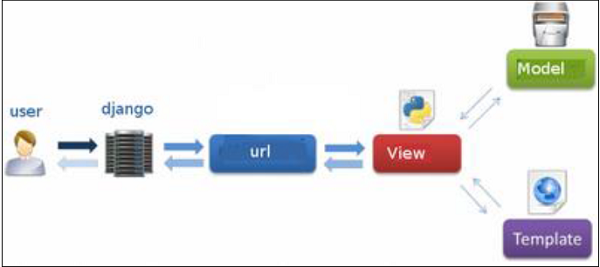
\includegraphics[width=12cm,height=6cm]{django1.png}\\
\subsection{Build Tool}

Ως Build και Deployment Tool θα χρησιμοποιήσουμε Docker Container.

\subsection{Διασύνδεση με Υπηρεσία Τοποθεσίας}

Google Maps Javascript API.

\subsection{HTTPS}

Η εφαρμογή θα τρέχει πάνω από SSL protocol.

\subsection{Communication/ Synchronization/ Version Control}

Χρήση Git Private Repository για την ανάπτυξη της εφαρμογής. 

\subsection{Watermark Placement}

Για την τοποθέτηση υδατογραφήματος στις φωτογραφίες των παρόχων θα χρησιμοποιηθεί η βιβλιοθήκη επεξεργασίας εικόνων Pillow της Python.


\subsection{Frontend - Οπτικοποίηση - WireFrames}

Τα templates της σελίδας βασίζονται σε Bootstrap 4 ενώ για τον σχεδιασμό του front end γίνεται χρήση JavaScript Libraries.
Tα Wireframes που θα χρησιμοποιήσουμε ως βάση είναι τα κάτωθι:\\
\includegraphics[width=12cm,height=8cm]{pic1.png}\\
\includegraphics[width=12cm,height=8cm]{pic2.png}\\
\includegraphics[width=12cm,height=8cm]{pic3.png}

\subsection{Flowcharts Xρηστών}
\includegraphics[width=12cm,height=8cm]{flow_1.png} \\
\includegraphics[width=12cm,height=8cm]{flow_2.png} \\
\includegraphics[width=12cm,height=8cm]{flow_3.png} \\

\end{document}
